\setlength{\parindent}{2em}

\section{Introduction}
\indent Certain physiological mechanisms that drive biological processes follow periodic synchronizations or rhythms. Examples of such phenomena include our heartbeats, the circadian rhythm, the menstrual cycle, hormone regulation, oscillating neurons, and more. While disruption or dysregulation of proper biological rhythms has been associated with diseases, induced perturbations to these oscillating systems (via a pacemaker or administration of therapeutic drugs) can reset the dynamics back to normal states\supercite{Glass2001}. 
\indent In 1994, Glass \& Sun\supercite{GLASS1994} mathematically approximated the effects of periodic pulsatile stimulations to cardiac oscillations using the Poincaré oscillator. The oscillator is a 2D vector in an abstract state space using polar coordinates ($r$, $\phi$) with $0\leq \phi \leq 1$, that evolves with time according to

\begin{align}
   \frac{\partial r}{\partial t} &= kr(1-r)\\ \frac{\partial \phi}{\partial t}&=1
\end{align}

\noindent where $r$ is the radial coordinate, $\phi$ is the angular coordinate, $k$, the relaxation rate which represents the rate of the system's return to the limit cycle at $r=1$. This evolution is periodically interrupted by a horizontal perturbation of magnitude $b$ every $\tau$ units of time. Initially a point ($r_i$, $\phi_i$) is perturbed horizontally by an amount $b$ to ($r'_i$,$\phi'_i$), 

\begin{align}
    r'&=\sqrt{r^2+b^2-2rb\cos(\pi-\phi 2\pi)}\\
     &=\sqrt{r^2+b^2+2rb\cos(\phi 2\pi)} 
     \label{eq: r}.
\end{align}

then ($r'_i$, $\phi'_i$) is evolved according to the differential equations for a time $\tau$ arriving at the point ($r_{i+1}$, $\phi_{i+1}$) (see Fig \ref{osc}). One can solve these differential equations explicitly to get a 2-dimensional map relating the points before and after the perturbation, $(r_i, \phi_i)$ and $(r_{i+1}, \phi_{i+1})$.

\begin{equation}
    r_{i+1} = \frac{r'_i}{(1 - r'_i)e^{-k\tau}+r'_i}
    \label{eqn:1}
\end{equation}

\begin{equation}
    \textnormal{mod} \{\phi_{i+1} = \phi_i' + \tau,1\}
    \label{eqn:2}
\end{equation}

The authors evaluated the organization of the model’s phase-locking regions as a function of parameters (\emph{b}, $\tau$, \emph{k}). Regions known as Arnold tongues, represent the different zones in (\emph{b}, $\tau$) space where a stable periodic oscillation exists for a particular ratio for the number of stimuli per period (period \#), to the number of complete revolutions in phase $\phi$, (cycle \#).

\begin{figure}[hbt!]
    \begin{center}
    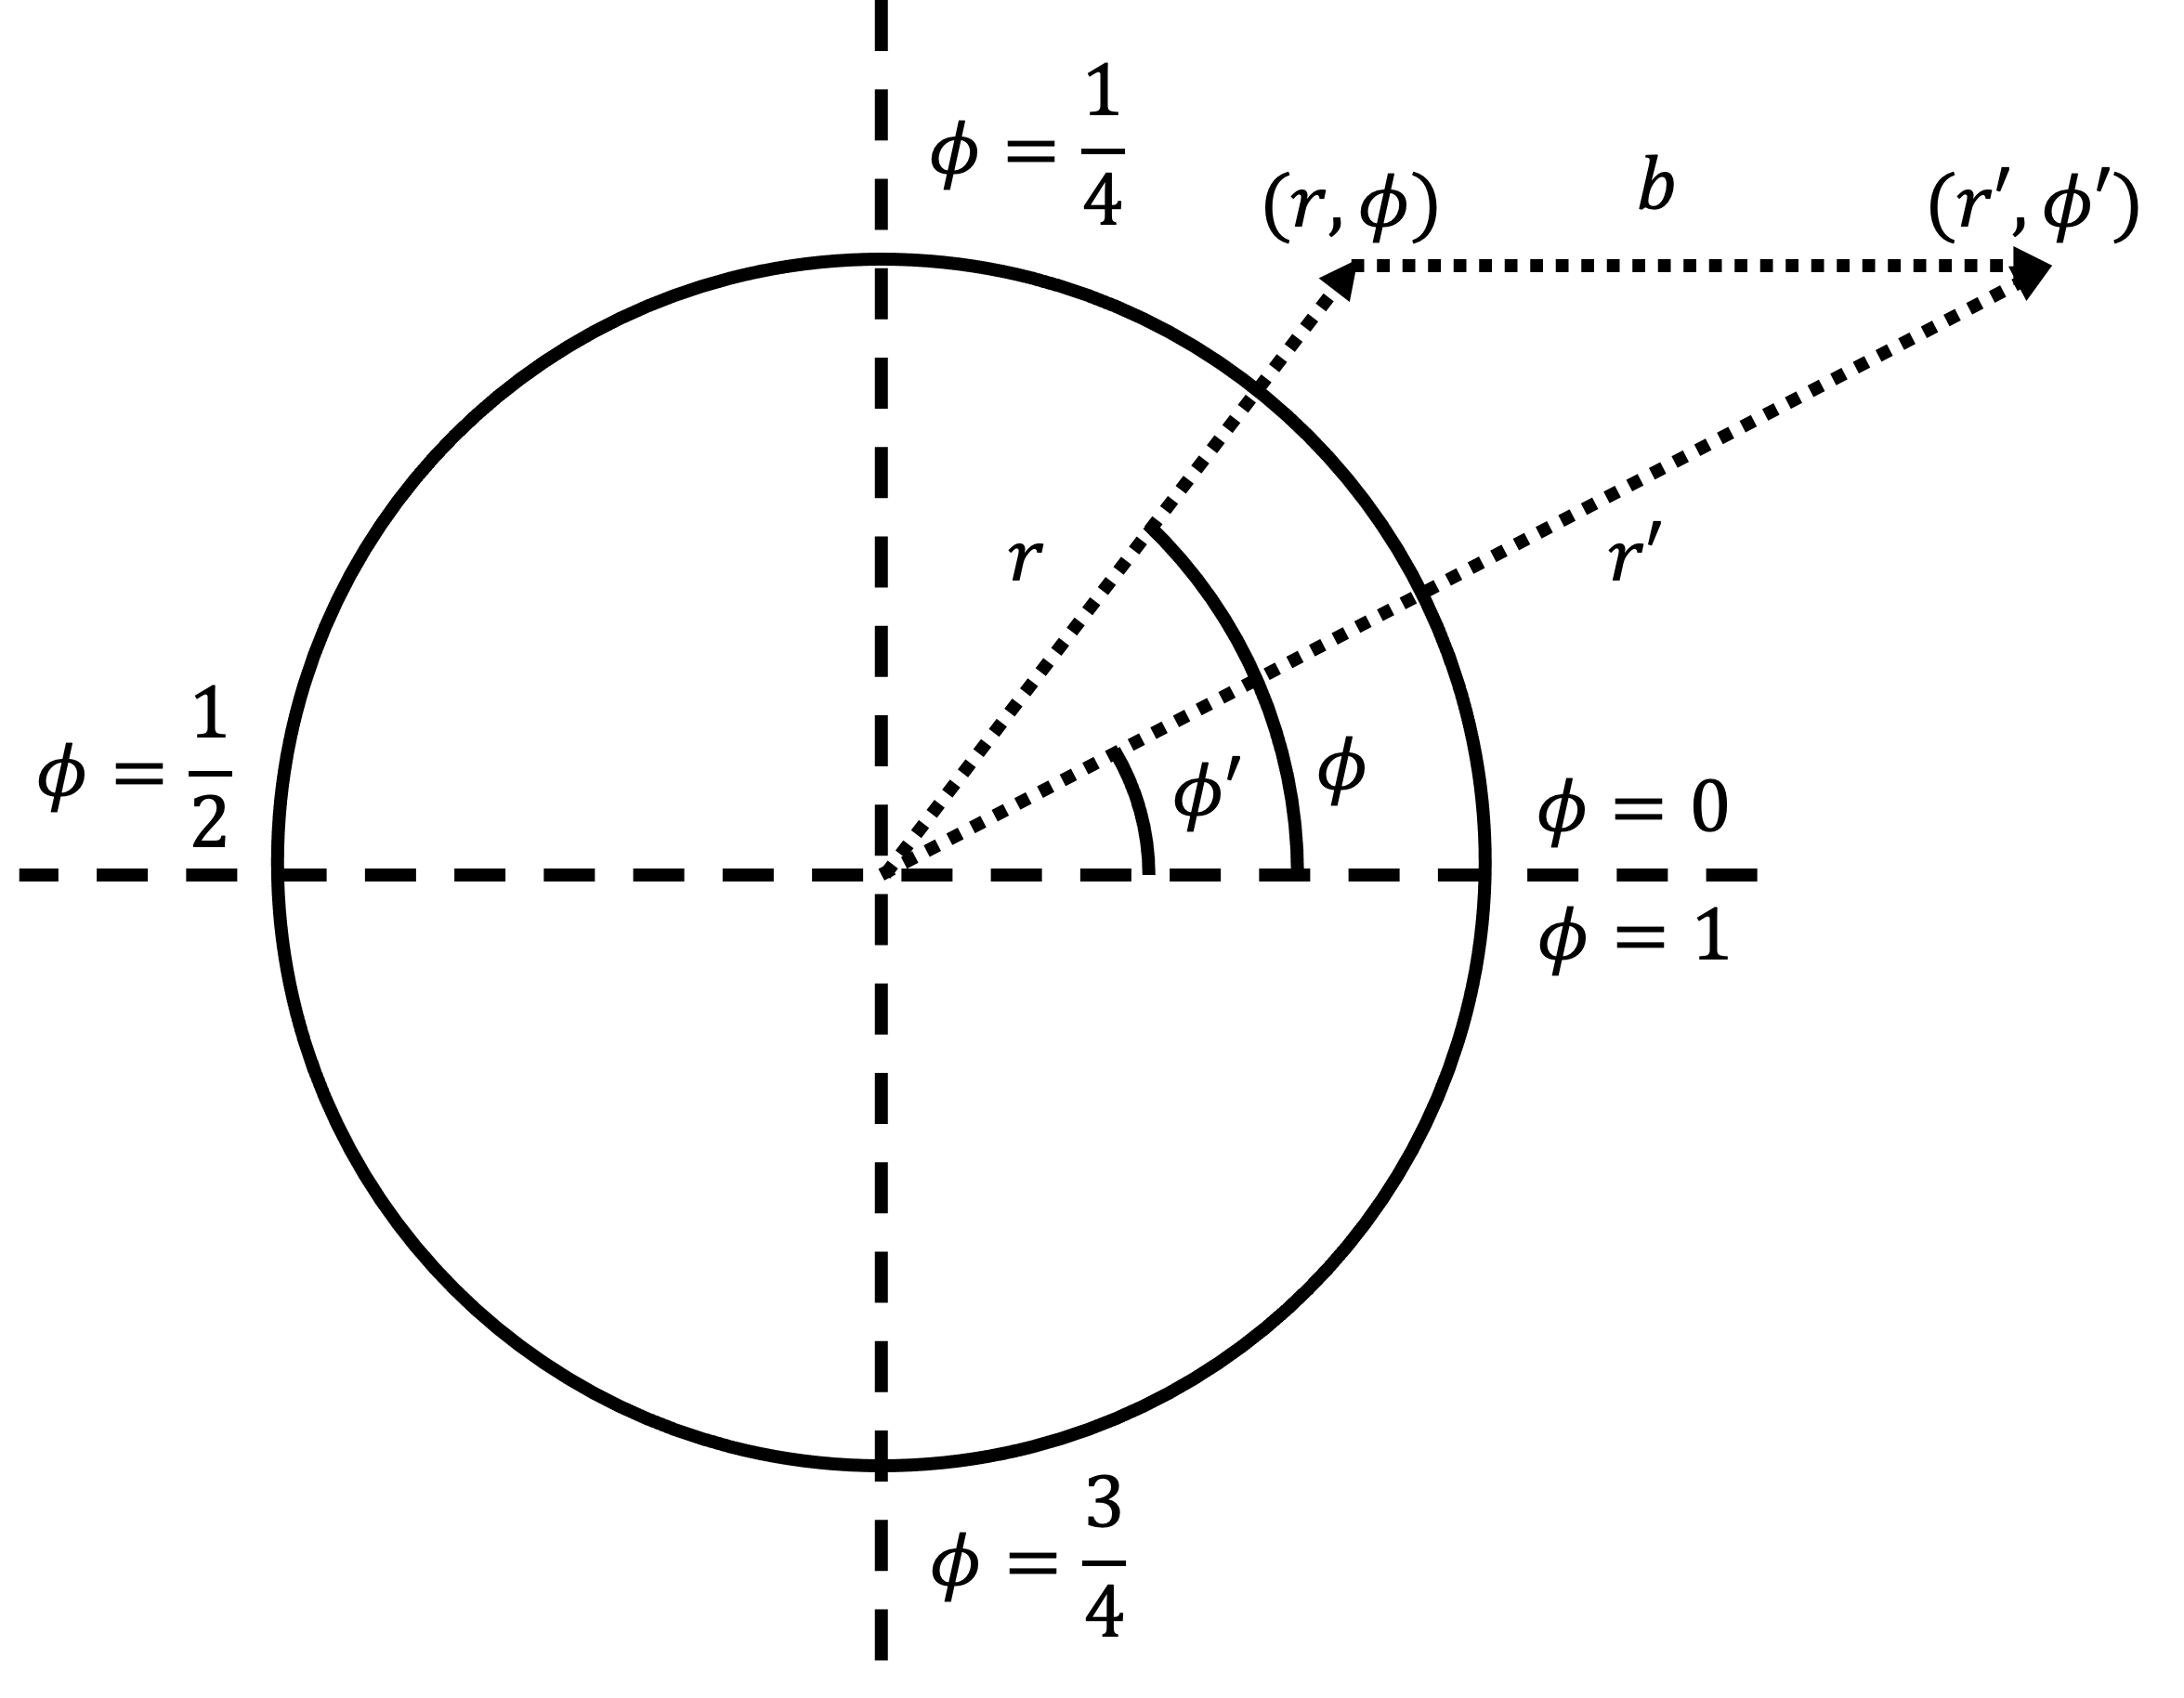
\includegraphics[width=.7\textwidth]{figures/Fig1.png}
    \end{center}
    \caption{A diagram of the oscillator, as seen in Glass \& Sun \cite{GLASS1994} Figure 1.}
    \label{osc}
\end{figure}

\indent In this study, we successfully replicate the complex dynamical behaviour observed by Glass \& Sun (1994)\supercite{GLASS1994} resulting from only two uncoupled ordinary differential equations and periodic forcing. This replication study is significant because 1) it numerically describes how finite relaxation rate back to the limit cycle affects the complex organization of the phase-locking regions and 2) because it analytically clarifies aspects of the instability boundary along the 1:0 and 1:1 (period \#: cycle \#) phase-locking regions in the infinite relaxation limit $(k \xrightarrow{} \infty$).

\section{Numerical Methods}
\indent We were able to replicate Glass \& Sun (1994)\supercite{GLASS1994} results in the programming language Julia version 1.7.2.
To overcome the model failure due to small numerical inaccuracies from rounding, we simulate the dynamics of this system by using the equations (\ref{eqn:1}) \& (\ref{eqn:2}) transformed into Cartesian coordinates with the form ($x_i$, $y_i$)\supercite{Glass2017}:

\begin{equation}
    x_{i+1} = \frac{(x_i + b)\cos(2\pi\tau) - y_i \sin(2\pi\tau)}{(1 - r'_i)e^{-k\tau}+r'_i}
    \label{eqn:7}
\end{equation}

\begin{equation}
    y_{i+1} = \frac{y_i \cos(2\pi\tau) + (x_i + b) \sin(2\pi\tau)}{(1-r'_i)e^{-k\tau} + r'_i}
    \label{eqn:8}
\end{equation}

where

\begin{equation}
    r'_i = [(x_i + b)^2 + y^2_i]^{1/2} \nonumber 
\end{equation}

This resolves the issue of round-off errors when $r_i \approx 1$, $b \approx 1$, and $\phi_i \approx 0.5$. In order to visually compare our results with the original paper, we then convert the Cartesian coordinates back into Polar coordinates.

We use initial values $x = 1$, $y = 0$, and $\phi = 0$ for $k=50\approx \infty$ to replicate Figure 2 of Glass \& Sun (1994)\supercite{GLASS1994}. These coordinates correspond to the fiducial point of the cycle at $r = 1$ and $\phi = 0$. The model is simulated over a period of 800 time-steps, although we only consider the periodic cycles after a 500 transient time had passed.

We compare the global organization of phase-locking regions for different values of $b$ and $\tau$ at $k=50\approx \infty$, $k = 10$, and $k = 1$. For $k$ evaluated at $10$ and $1$, we use the initial points ($x = -0.30810803127799$, $y = 0.95135137623383$) which correspond to the arbitrarily chosen initial states ($r = 1$, $\phi = 0.3$) of the original paper. Furthermore, to investigate the dynamics at specific regions of the phase-locking zones, we produce figures zoomed in at $\tau = 0.25$ and $b = 1$, as well as at $\tau = 0.35$ and $b = 1$.

Figures show the phase-locking zones between the number of stimuli per period (denoted \emph{period n}) for 1 cycle, in an $n:1$ ratio.

\begin{figure}[tbph]

\centering
        \subfloat[]{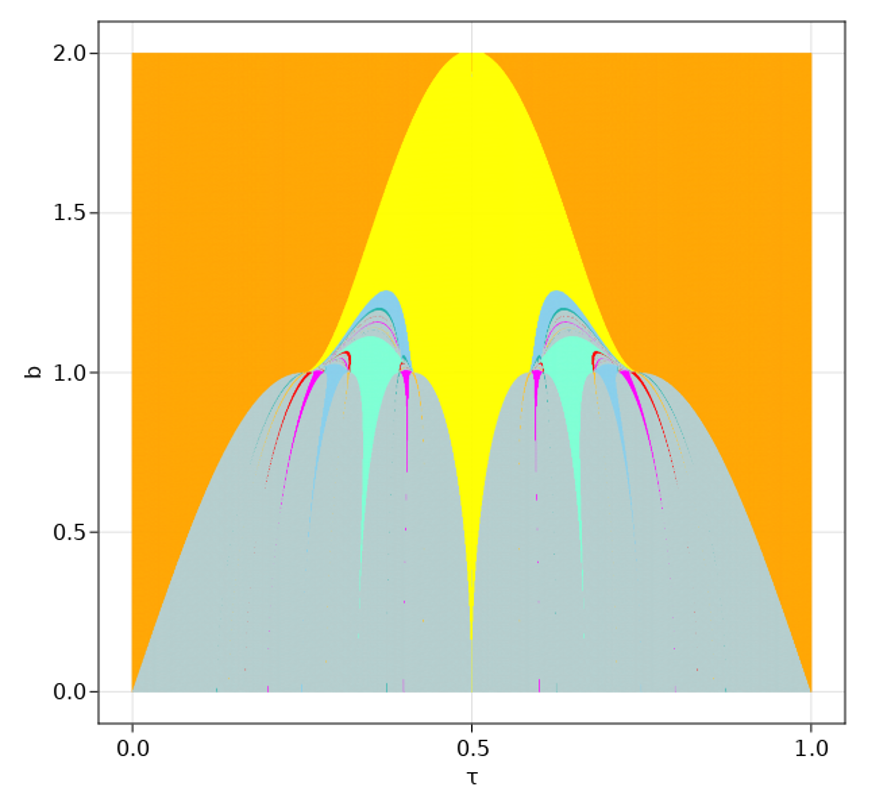
\includegraphics[width=0.45\textwidth]{figures/k50_1.png}\label{fig:a}}
    \medskip
        \subfloat[]{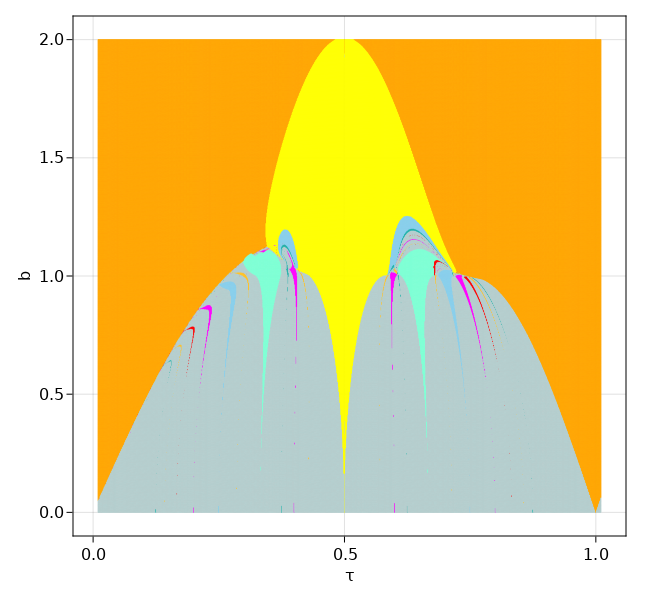
\includegraphics[width=0.45\textwidth]{figures/k10.png}\label{fig:b}}
    \hfil
        \subfloat[]{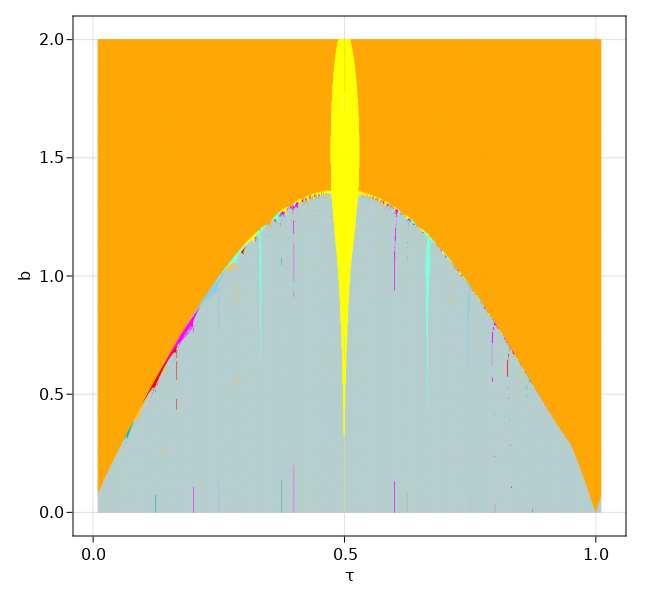
\includegraphics[width=0.45\textwidth]{figures/k1.png}\label{fig:d}}
    \medskip
        \subfloat[]{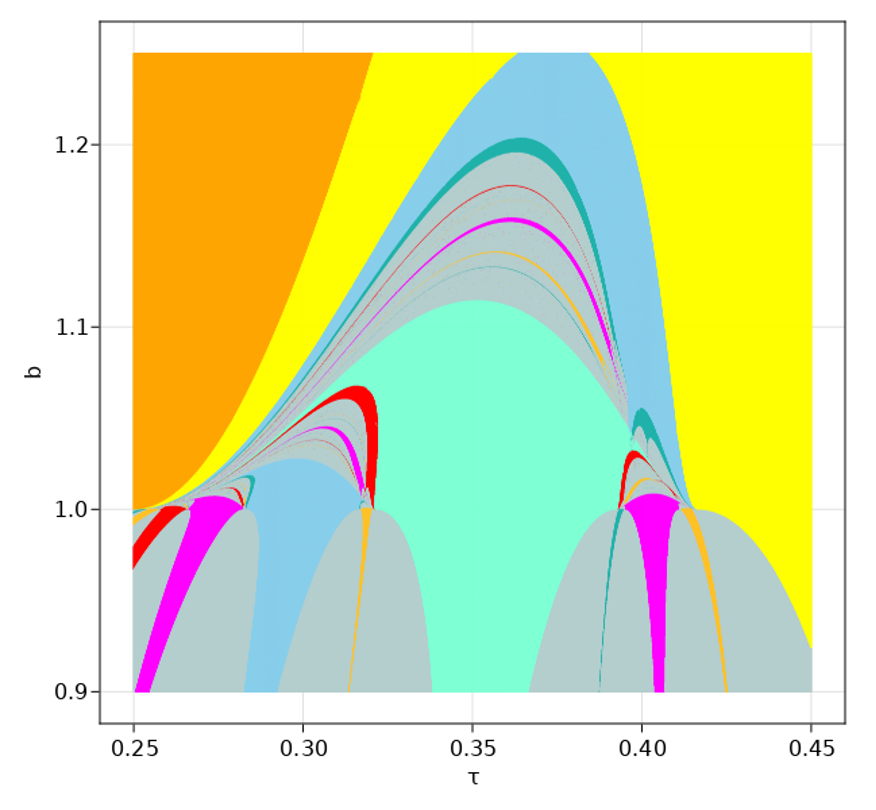
\includegraphics[width=0.45\textwidth]{figures/k50_2.png}\label{fig:e}}
    \hfil
        \subfloat[]{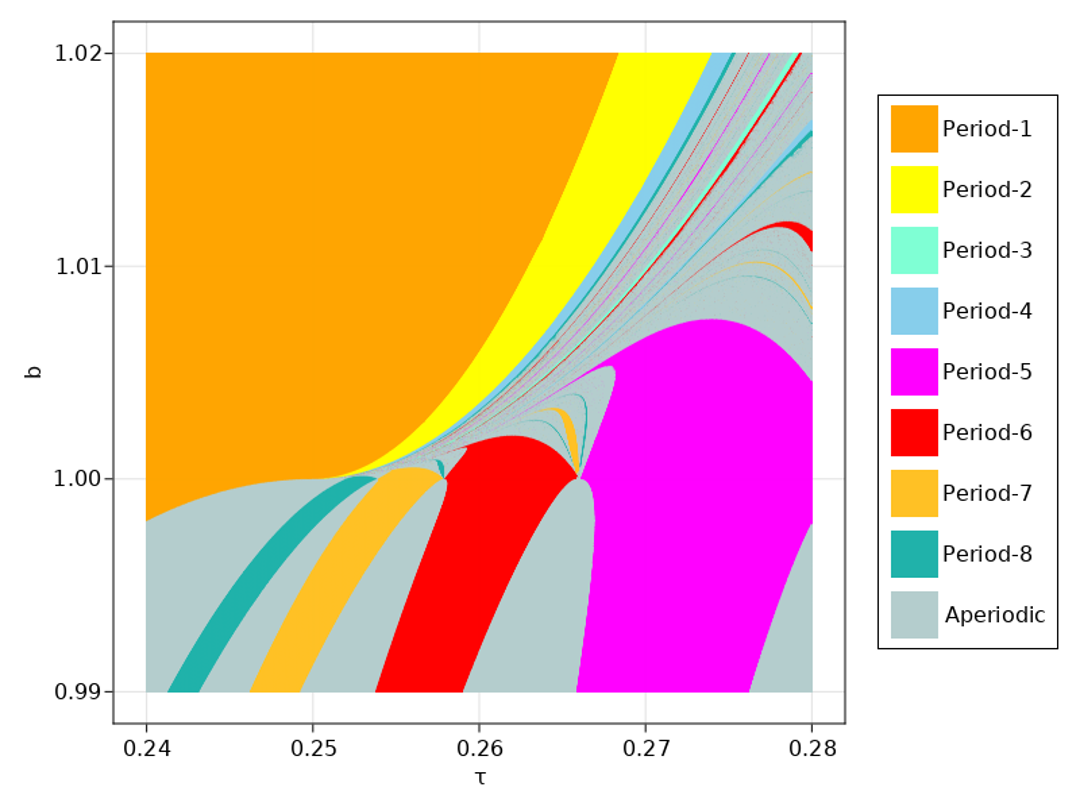
\includegraphics[width=0.6\textwidth]{figures/k50_3.png}\label{fig:f}}
    
\caption{\textbf{Global organization of phase-locking zones of the periodically forced oscillator for different relaxation rate}. We demonstrate organization of the phase-locking zones for (a) $k$ infinite; (b) $k = 10$; (c) $k = 1$; (d) $k$ infinite at increased resolution at point $\tau = 0.25$ and $b = 1.0$; (e) $k$ infinite at increased resolution at point $\tau = 0.35$ and $b = 1$. We show the $n:1$ locked period-cycles for different frequencies of stimulus $\tau$ and magnitude of stimulus $b$, as aforementioned in the text. We were able to successfully reproduce corresponding Figure 2, Figure 5a and Figure 5b of the original study. Despite the expected minor differences, our results follow the same overall patterns.}
    \label{replic}
\end{figure}

%\caption{Phase locking zones for the oscillator. The grey region labelled aperiodic could include stable cycles of period nine or greater, or truly aperiodic dynamics. $k=50$.}

\section{Analytical Results}
\indent Our goal is to analytically calculate the period-1 instability boundary in the immediate relaxation limit ($k \rightarrow \infty$). $k \rightarrow \infty$ is called the immediate relaxation limit as the system returns (in the radial direction) to the limit cycle at $r=1$ immediately after the perturbation; all time evolution occurs on the unit circle and the 2D map reduces to a 1D map described by $\phi_{i+1}(\phi_i, b, \tau)$. The period-1 instability boundary is determined by setting $\phi_{i+1} = \textnormal{mod} \{\phi_i,1\}$ (period-1 condition) and $|\frac{\partial \phi_{i+1}}{\partial \phi_i}|>1$ (instability condition). $|\frac{\partial \phi_{i+1}}{\partial \phi_i}|>1$ translates to small deviations from the fixed point becoming larger after applications of the 1D map (see pg. 356 in Strogatz\supercite{Strogatz}). The period-1 instability boundary in the immediate relaxation limit (along with other instability boundaries) is shown in Fig. \ref{replic}.

Using the law of cosines and noting $\angle{rb}= \pi-\phi 2\pi$ (see Fig. \ref{osc}), the radial coordinate $r'(r,\phi,b)$ after perturbation is:
\begin{align}
    r'&=\sqrt{r^2+b^2-2rb\cos(\pi-\phi 2\pi)}\\
     &=\sqrt{r^2+b^2+2rb\cos(\phi 2\pi)} 
     \label{eq: r}.
\end{align}
Again, using the law of cosines (see Fig. \ref{osc}), the angular coordinate $\phi'(r,\phi,b)$ after perturbation is:
\begin{align}
    r &=\sqrt{r'^2+b^2-2r'b\cos(\phi' 2\pi)} \\
    \cos(\phi' 2\pi) &= \frac{r^2+b^2+2rb\cos(\phi 2\pi) +b^2 - r^2}{2r'b} \\
    &= \frac{b+r \cos(\phi 2\pi)}{\sqrt{r^2+b^2+2rb\cos(\phi 2\pi)}} \\
    \phi' &= \frac{1}{2\pi}\arccos(\frac{b+r \cos(\phi 2\pi)}{\sqrt{r^2+b^2+2rb\cos(\phi 2\pi)}})
\end{align} where Eq. \ref{eq: r} is used in line 9 and line 10. However, $\arccos(\cos(2\pi \phi')) = 2\pi \phi'$ only if $0\leq \phi' \leq 1/2$. This is because arccosine only inverts the first half-period of cosine function between $0$ to $\pi$. For $1/2 \leq \phi' \leq 1$, we note that $-\arccos(\cos(2\pi \phi')) +2\pi= 2\pi \phi'$. So over the complete range of possible perturbed phases, we have:
\begin{equation}
    \phi' =
    \begin{cases}
     \frac{1}{2\pi}\arccos(\frac{b+r \cos(\phi 2\pi)}{\sqrt{r^2+b^2+2rb\cos(\phi 2\pi)}}) & 0 \leq \phi' \leq 1/2 \\
    -\frac{1}{2\pi}\arccos(\frac{b+r \cos(\phi 2\pi)}{\sqrt{r^2+b^2+2rb\cos(\phi 2\pi)}}) + 1 & 1/2 \leq \phi' \leq 1 \\
    \end{cases}
\end{equation}

As $\tau$ is increased from 0, the curve intersects the line $\phi_{i+1}= \phi_i$ tangentially. Hence, the type of bifurcation for the period-1 instability boundary is a tangent bifurcation. Integrating the angular differential equation is trivial: $\phi_{i+1} = \textnormal{mod} \{\phi'_i + \tau,1\}$, which adds $\tau$ to the above piecewise equation. Note that since the perturbations are horizontal, if $0 \leq \phi \leq 1/2$, then $0 \leq \phi' \leq 1/2$; and if $1/2 \leq \phi \leq 1$, then $1/2 \leq \phi' \leq 1$ (the perturbation never causes the system to cross the x-axis). It is useful to rewrite $\phi_{i+1}(r_i=1,\phi_i,b,\tau)$ in a different form, which makes it easier to calculate the derivative $\frac{\partial \phi_{i+1}}{\partial \phi_i}$.

\indent We begin by noting that $\arccos(x) = \cot^{-1}(\frac{x}{\sqrt{1-x^2}})$ for $|x|<1$ which is always satisfied for any $\phi$, $b$, $r$, if $x=\frac{b+r \cos(\phi_i 2\pi)}{\sqrt{r^2+b^2+2rb\cos(\phi_i 2\pi)}}$. 

Then, 
\begin{align}
    \frac{x}{\sqrt{1-x^2}} &= \frac{\frac{b+r_i \cos(\phi_i 2\pi)}{\sqrt{r_i^2+b^2+2r_b\cos(\phi_i 2\pi)}}}{\sqrt{1-(\frac{b+r_i \cos(\phi_i 2\pi)}{\sqrt{r_i^2+b^2+2r_i b\cos(\phi_i 2\pi)}})^2}} & r_i = 1 \nonumber \\
    &= \frac{b + \cos(2\pi \phi_i)}{\sin(2\pi \phi_i)} \nonumber \\
    &= b\csc(2\pi \phi_i) + \cot(2\pi \phi_i)
\end{align} 
Gives, 
\begin{equation}
    \phi_{i+1} =
\begin{cases}
        \frac{1}{2\pi}\cot^{-1}(b\csc(2\pi \phi_i)+\cot(2\pi \phi_i))+ \tau & 0 \leq \phi_i \leq 1/2 \\
       -\frac{1}{2\pi}\cot^{-1}(b\csc(2\pi \phi_i)+\cot(2\pi \phi_i))+ \tau + 1 & 1/2 \leq \phi_i \leq 1 \\
    \end{cases}
\end{equation}
The derivative is then computed as:
%derivative
\begin{align}
    \phi_{i+1} &= \phi_i' + \tau \nonumber \\
    &= \frac{1}{2\pi}\cot^{-1}(b\csc(2\pi \phi_i)+\cot(2\pi \phi_i))+ \tau \nonumber \\
    \frac{\partial \phi_{i+1}}{\partial \phi_i} &= \frac{1}{2\pi} \frac{-\frac{\partial (b\csc(2\pi \phi_i)+\cot(2\pi \phi_i))}{\partial \phi_i}}{1+(b\csc(2\pi \phi_i)+\cot(2\pi \phi_i))^2} \nonumber \\
    &= \frac{1+b\cos(2\pi \phi_i)}{\sin^2(2\pi \phi_i)+\cos^2(2\pi \phi_i) + b^2 + 2b\cos(2\pi \phi_i)} \nonumber \\
    &=\frac{1+b\cos(2\pi \phi_i)}{1 + b^2 + 2b\cos(2\pi \phi_i)}.
\end{align}

\indent The general strategy to compute the instability is to set $\frac{\partial \phi_{i+1}}{\partial \phi_i} = \pm 1$ which will give an equation for $b(\phi_i)$. $b(\phi_i)$ can be substituted into $\phi_{i+1}(\phi_i,b,\tau)$; and setting $\phi_{i+1} = \phi_i$ (period-1 condition) gives $\phi_i(\tau)$. Finally, $\phi_i(\tau)$ is substituted into $b(\phi_i)$ resulting in the period-1 ($k\rightarrow \infty$) instability boundary $b(\tau)$.\\
We start by setting $\frac{\partial \phi_{i+1}}{\partial \phi_i} = 1$:
\begin{align}
    1 &= \frac{1+b\cos(2\pi \phi_i)}{1 + b^2 + 2b\cos(2\pi \phi_i)} & 0\leq \phi_i \leq 1/2 \nonumber \\
    b&= -\cos(2\pi \phi_i)
\end{align} 
Then, since $1/4 + \tau = \phi_{i+1} = \phi_i \leq 1/2$ implies $\tau \leq 1/4$:

\begin{equation}
    \phi_{i+1} = \phi_i = \frac{1}{2\pi}\arccos(\frac{b+\cos(\phi_i 2\pi)}{\sqrt{1+b^2+2b\cos(\phi_i 2\pi)}}) + \tau = \frac{1}{2\pi}\arccos(0) + \tau = 1/4 +\tau
\end{equation}

\noindent Where,
\begin{align}
    b&= -\cos(2\pi \phi_i) \nonumber \\
    &= -\cos(2\pi(1/4 +\tau)) & 0 \leq \phi_i \leq 1/2 \nonumber \\
    &= \sin(2\pi\tau) & \tau \leq 1/4
\end{align} 
For $1/2 \leq \phi \leq 1$, since $1/2 \leq 3/4 + \tau = \phi_{i+1} = \phi_i $ implies $ \textnormal{mod} \{-1/4,1\} \leq \tau $ then $ \tau \geq 3/4$:

\begin{equation}
    \phi_{i+1} = \phi_i = -\frac{1}{2\pi}\arccos(\frac{b+\cos(\phi_i 2\pi)}{\sqrt{1+b^2+2b\cos(\phi_i 2\pi)}}) + 1 + \tau = -\frac{1}{2\pi}\arccos(0) + 1 + \tau = 3/4 +\tau
\end{equation}

\noindent Where,
\begin{align}
b&= -\cos(2\pi \phi_i) \nonumber \\
&= -\cos(2\pi(3/4 +\tau)) & 1/2 \leq \phi_i \leq 1 \nonumber \\
&= -\sin(2\pi\tau) & \tau \geq 3/4
\end{align}

\noindent In summary, $b = |\sin(2\pi\tau)|$ for $\tau \leq 1/4$ and $\tau \geq 3/4$.

\noindent We can also set $\frac{\partial \phi_{i+1}}{\partial \phi_i} = -1$:
\begin{align}
    -1 &= \frac{1+b\cos(2\pi \phi_i)}{1 + b^2 + 2b\cos(2\pi \phi_i)} \nonumber \\
    0 &= 2+3b\cos(2\pi \phi_i) + b^2 \nonumber \\
    \frac{-b^2-2}{3b} &= \cos(2\pi \phi_i)
    \label{eq:square} 
\end{align}
The phase response curve for this instability is then:
\begin{align}
    \phi_{i+1} = \phi_i &= \frac{1}{2\pi}\arccos(\frac{b+\frac{-b^2-2}{3b}}{\sqrt{1+b^2+2b\frac{-b^2-2}{3b}}}) + \tau \nonumber \\
    2\pi(\phi_i - \tau) &= \arccos(\frac{2\sqrt{1/3*(b^2-1)}}{b})
\end{align} 
We make use of the identity $\arccos(x) = \arcsin(\sqrt{1-x^2})$, which holds for $b>1$, with $x = \frac{2\sqrt{1/3*(b^2-1)}}{b}$, for reasons that will become clear shortly. $\sqrt{1-x^2}$ is then $\sqrt{1-\frac{4(b^2-1)}{3b^2}} = \sqrt{\frac{3b^2-4b^2+4}{3b^2}} = \sqrt{\frac{-b^2+4}{3b^2}}$. $2\pi(\phi_i - \tau) = \arcsin(\sqrt{\frac{-b^2+4}{3b^2}})$ so $\phi_i = \tau +\frac{1}{2\pi}\arcsin(\sqrt{\frac{-b^2+4}{3b^2}})$, which agrees with Section C of Glass \& Sun \supercite{GLASS1994}.

%diagram for k->\infty
\indent In order to proceed, we refer to the geometry of the period-1 cycle. Referring to Fig. \ref{sines}, the law of sines gives $\frac{\sin(2\pi \tau)}{b}=\frac{\sin(2\pi \phi'_i)}{r_i}=\frac{\sin(2\pi (\phi_i -\tau))}{r_i}$ for $0\leq \phi \leq1/2$ and $\frac{\sin(2\pi \tau)}{b}=\frac{\sin(2\pi (1-\phi'_i))}{r_i}=-\frac{\sin(2\pi \phi'_i)}{r_i}=-\frac{\sin(2\pi (1+\phi_i-\tau))}{r_i}=-\frac{\sin(2\pi (\phi_i-\tau))}{r_i}$ for $1/2\leq \phi \leq1$. Note $r_i=1$ for $k\rightarrow \infty$. This can be used to simplify:
\begin{align}
    2\pi(\phi_i - \tau) &= \arcsin(\sqrt{\frac{-b^2+4}{3b^2}}) \nonumber \\
    \pm\frac{\sin(2\pi \tau)}{b} &= \sin(\arcsin(\sqrt{\frac{-b^2+4}{3b^2}}))\nonumber \\
    (\pm\frac{\sin(2\pi \tau)}{b})^2 &= \frac{-b^2+4}{3b^2} \nonumber \\
    b &= \sqrt{4-3\sin^2(2\pi\tau)} 
    \label{eq:bound2}
\end{align}
Next we check if there are any restrictions on $\tau$ for which $b = \sqrt{4-3\sin^2(2\pi\tau)}$ is not a period-1 instability boundary. Using the identity $\sin^2(2\pi\tau) + \cos^2(2\pi\tau) = 1$ and solving for $\tau$ we find:
\begin{align}
    b &= \sqrt{4-3(1-\cos^2(2\pi\tau))}\\
    \tau &= \frac{1}{2\pi}\arccos(\pm\sqrt{(b^2 - 1)/3}).
\end{align}
Since $\arccos(\cos(2\pi \tau)) = 2\pi \tau$ only if $0 \leq \tau \leq 1/2$ and $-\arccos(\cos(2\pi \tau)) +2\pi= 2\pi \tau$, for $1/2 \leq \tau \leq 1$, we can write:
\begin{equation} 
\tau =
\begin{cases}
        \frac{1}{2\pi}\arccos(\pm\sqrt{(b^2 - 1)/3}) & 0 \leq \tau \leq 1/2, 0 \leq \phi_i \leq 1/2 \\
       -\frac{1}{2\pi}\arccos(\pm\sqrt{(b^2 - 1)/3}) + 1 & 1/2 \leq \tau \leq 1, 1/2 \leq \phi_i \leq 1
    \end{cases}
\end{equation} Note that $0 \leq \tau \leq 1/2$ implies $0 \leq \phi_i \leq 1/2$ for the period-1 cycle, which can be checked using $\tau = \phi_i - \phi'_i$ and $\phi'_i<\phi_i$. Similarly $1/2 \leq \tau \leq 1$ implies $1/2 \leq \phi \leq 1$ which can be checked using $\tau = 1-(\phi'_i - \phi_i)$ and $\phi'_i>\phi_i$.\\

\noindent Combing this result with the phase response curve, we get:
\begin{equation} \phi_{i+1} =
\begin{cases}
        \frac{1}{2\pi}\arccos(\frac{b+\cos(\phi_i 2\pi)}{\sqrt{1+b^2+2b\cos(\phi_i 2\pi)}}) + \frac{1}{2\pi}\arccos(\pm\sqrt{(b^2 - 1)/3}) & 0 \leq \phi_i \leq 1/2 \\
       -\frac{1}{2\pi}\arccos(\frac{b+\cos(\phi_i 2\pi)}{\sqrt{1+b^2+2b\cos(\phi_i 2\pi)}}) -\frac{1}{2\pi}\arccos(\pm\sqrt{(b^2 - 1)/3}) + 2& 1/2 \leq \phi_i \leq 1. \\
    \end{cases}
\end{equation}
However, when $1\leq b$, the period-1 condition $\phi_{i+1} = \textnormal{mod} \{\phi'_i + \tau,1\}$ at the instability boundary $\frac{\partial \phi_{i+1}}{\partial \phi_i} = -1$, is satisfied only for Eq \ref{eq:satisf} and not for Eq \ref{eq:reject}.

\begin{equation} 
    \tau =
    \begin{cases}
        \frac{1}{2\pi}\arccos(-\sqrt{(b^2 - 1)/3}) & 0 \leq \phi_i \leq 1/2 \\
       -\frac{1}{2\pi}\arccos(-\sqrt{(b^2 - 1)/3}) + 1 & 1/2 \leq \phi_i \leq 1
    \end{cases}
    \label{eq:satisf}
\end{equation} 

\begin{equation} 
    \tau =
    \begin{cases}
        \frac{1}{2\pi}\arccos(+\sqrt{(b^2 - 1)/3}) & 0 \leq \phi_i \leq 1/2 \\
       -\frac{1}{2\pi}\arccos(+\sqrt{(b^2 - 1)/3}) + 1 & 1/2 \leq \phi_i \leq 1
    \end{cases}
    \label{eq:reject}
\end{equation} 

At the $\frac{\partial \phi_{i+1}}{\partial \phi_i} = -1$ instability boundary, the phase must be a solution of $0 = 2+3b\cos(2\pi \phi_i) + b^2$. The equation \ref{eq:right} is satisfied at the $\phi_i$ equal to the $\phi_i$ solutions of $0 = 2+3b\cos(2\pi \phi_i) + b^2$ while the equation \ref{eq:wrong} is satisfied for other $\phi_i$ values off the $\frac{\partial \phi_{i+1}}{\partial \phi_i} = -1$ instability boundary (see Fig \ref{instabbound}).

\begin{equation} 
    0 = 
    \begin{cases}
       \phi_i - \textnormal{mod} \{\frac{1}{2\pi}\arccos(\frac{b+\cos(\phi_i 2\pi)}{\sqrt{1+b^2+2b\cos(\phi_i 2\pi)}}) + \frac{1}{2\pi}\arccos(-\sqrt{(b^2 - 1)/3}),1\}& 0 \leq \phi_i \leq 1/2 \\
       \phi_i - \textnormal{mod} \{-\frac{1}{2\pi}\arccos(\frac{b+\cos(\phi_i 2\pi)}{\sqrt{1+b^2+2b\cos(\phi_i 2\pi)}})-\frac{1}{2\pi}\arccos(-\sqrt{(b^2 - 1)/3}) + 2,1\}& 1/2 \leq \phi_i \leq 1 \\
    \end{cases}
    \label{eq:right}
\end{equation} 

\begin{equation} 
    0 = 
    \begin{cases}
       \phi_i - \textnormal{mod} \{\frac{1}{2\pi}\arccos(\frac{b+\cos(\phi_i 2\pi)}{\sqrt{1+b^2+2b\cos(\phi_i 2\pi)}}) + \frac{1}{2\pi}\arccos(+\sqrt{(b^2 - 1)/3}),1\}& 0 \leq \phi_i \leq 1/2 \\
       \phi_i - \textnormal{mod} \{-\frac{1}{2\pi}\arccos(\frac{b+\cos(\phi_i 2\pi)}{\sqrt{1+b^2+2b\cos(\phi_i 2\pi)}})-\frac{1}{2\pi}\arccos(+\sqrt{(b^2 - 1)/3}) + 2,1\}& 1/2 \leq \phi_i \leq 1 \\
    \end{cases}
    \label{eq:wrong}
\end{equation} 

Therefore we reject Eq.(\ref{eq:reject}) as a solution to $\cos^2(2\pi\tau) = (b^2 - 1)/3$, which means $\cos(2\pi\tau) = -\sqrt{(b^2 - 1)/3}$ effectively restricts the period-1 instability boundary $b = \sqrt{4-3\sin^2(2\pi\tau)}$ to $1/4<\tau<3/4$, (see Fig \ref{instabbound_restric}).

\begin{figure}[H]
    \begin{center}
    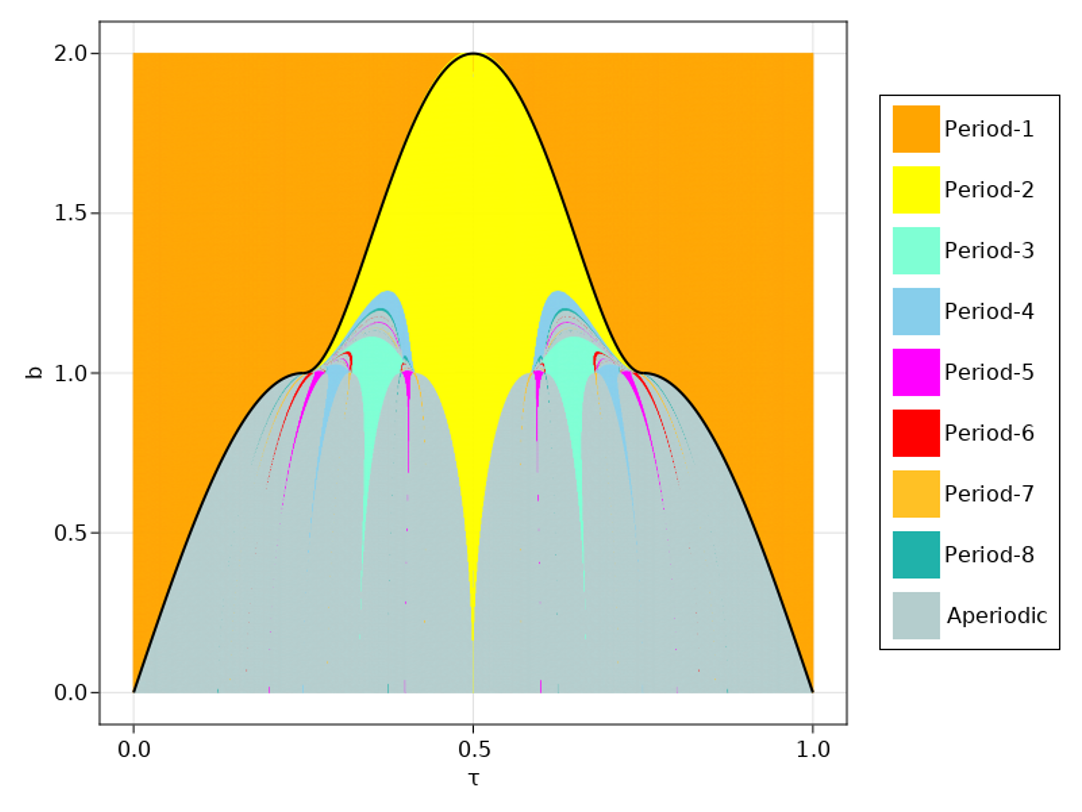
\includegraphics[width=.8\textwidth]{figures/k50_4.png}
    \end{center}
    \caption{Phase-locking zones for the oscillator, $k=50$, with $k\rightarrow \infty$ period-1 instability boundaries $b = |\sin(2\pi\tau)|$ ($\tau \leq 1/4$, $\tau \geq 3/4$) and $b = \sqrt{4-3\sin^2(2\pi\tau)}$ ($1/4<\tau<3/4$) in black.}
    \label{}
\end{figure}

Finally it should be noted that these calculations do not reveal the cycle number for either instability boundary.

\section{Conclusion}

In this study, we successfully replicate the dynamics of the periodic forcing of an oscillator from the original paper by Glass \& Sun \supercite{GLASS1994}. We plot the phase‐locking regions for varying relaxation limits and algebraically compute the boundaries of the 1:1 phase-locking rhythm, as the infinite relaxation limit loses stability and determined a tangent bifurcation. Additionally, we visually show the solutions of the instability boundaries, as seen in the supplementary figures section. 